%% 
%% Copyright 2007-2020 Elsevier Ltd
%% 
%% This file is part of the 'Elsarticle Bundle'.
%% ---------------------------------------------
%% 
%% It may be distributed under the conditions of the LaTeX Project Public
%% License, either version 1.2 of this license or (at your option) any
%% later version.  The latest version of this license is in
%%    http://www.latex-project.org/lppl.txt
%% and version 1.2 or later is part of all distributions of LaTeX
%% version 1999/12/01 or later.
%% 
%% The list of all files belonging to the 'Elsarticle Bundle' is
%% given in the file `manifest.txt'.
%% 
%% Template article for Elsevier's document class `elsarticle'
%% with harvard style bibliographic references

%\documentclass[preprint,12pt,authoryear]{elsarticle}

%% Use the option review to obtain double line spacing
%% \documentclass[authoryear,preprint,review,12pt]{elsarticle}

%% Use the options 1p,twocolumn; 3p; 3p,twocolumn; 5p; or 5p,twocolumn
%% for a journal layout:
%% \documentclass[final,1p,times,authoryear]{elsarticle}
%% \documentclass[final,1p,times,twocolumn,authoryear]{elsarticle}
%% \documentclass[final,3p,times,authoryear]{elsarticle}
%% \documentclass[final,3p,times,twocolumn,authoryear]{elsarticle}
%% \documentclass[final,5p,times,authoryear]{elsarticle}
 \documentclass[final,5p,times,twocolumn]{elsarticle}
 \makeatletter
\def\ps@pprintTitle{%
     \let\@oddhead\@empty
     \let\@evenhead\@empty
     \def\@oddfoot{}%
     \let\@evenfoot\@oddfoot}
\makeatother


%% For including figures, graphicx.sty has been loaded in
%% elsarticle.cls. If you prefer to use the old commands
%% please give \usepackage{epsfig}

%% The amssymb package provides various useful mathematical symbols
\usepackage{amssymb}
\usepackage{lipsum}
%% The amsthm package provides extended theorem environments
%% \usepackage{amsthm}

%% The lineno packages adds line numbers. Start line numbering with
%% \begin{linenumbers}, end it with \end{linenumbers}. Or switch it on
%% for the whole article with \linenumbers.
%% \usepackage{lineno}

%% You might want to define your own abbreviated commands for common used terms, e.g.:
\newcommand{\kms}{km\,s$^{-1}$}
\newcommand{\msun}{$M_\odot}

\begin{document}

\begin{frontmatter}

\title{Transformers usecases in biology}
\author[first]{Lena Trnovec}
\end{frontmatter}


\section{Introduction}
\label{introduction}

TODO
\section{Encoding proteins as vectors in a high-dimensional space}
Transformers have been used to encode proteins as vectors in a high-dimensional space, where sequences with similar properties are mapped closely together. This study~\cite{rives_biological_2021} demonstrates that after training, the representation space of a transformer model clusters orthologous genes effectively. This is visualized through t-SNE and PCA (figure \ref{fig:gene-tsne}), which show that species and orthology become principal axes of variation, indicating that unsupervised learning captures biological variations. This learned structure allows for improved recovery of proteins based on biological properties using vector similarity queries, confirming that biological information is encoded within the representation space.
\begin{figure}[ht]
    \centering
    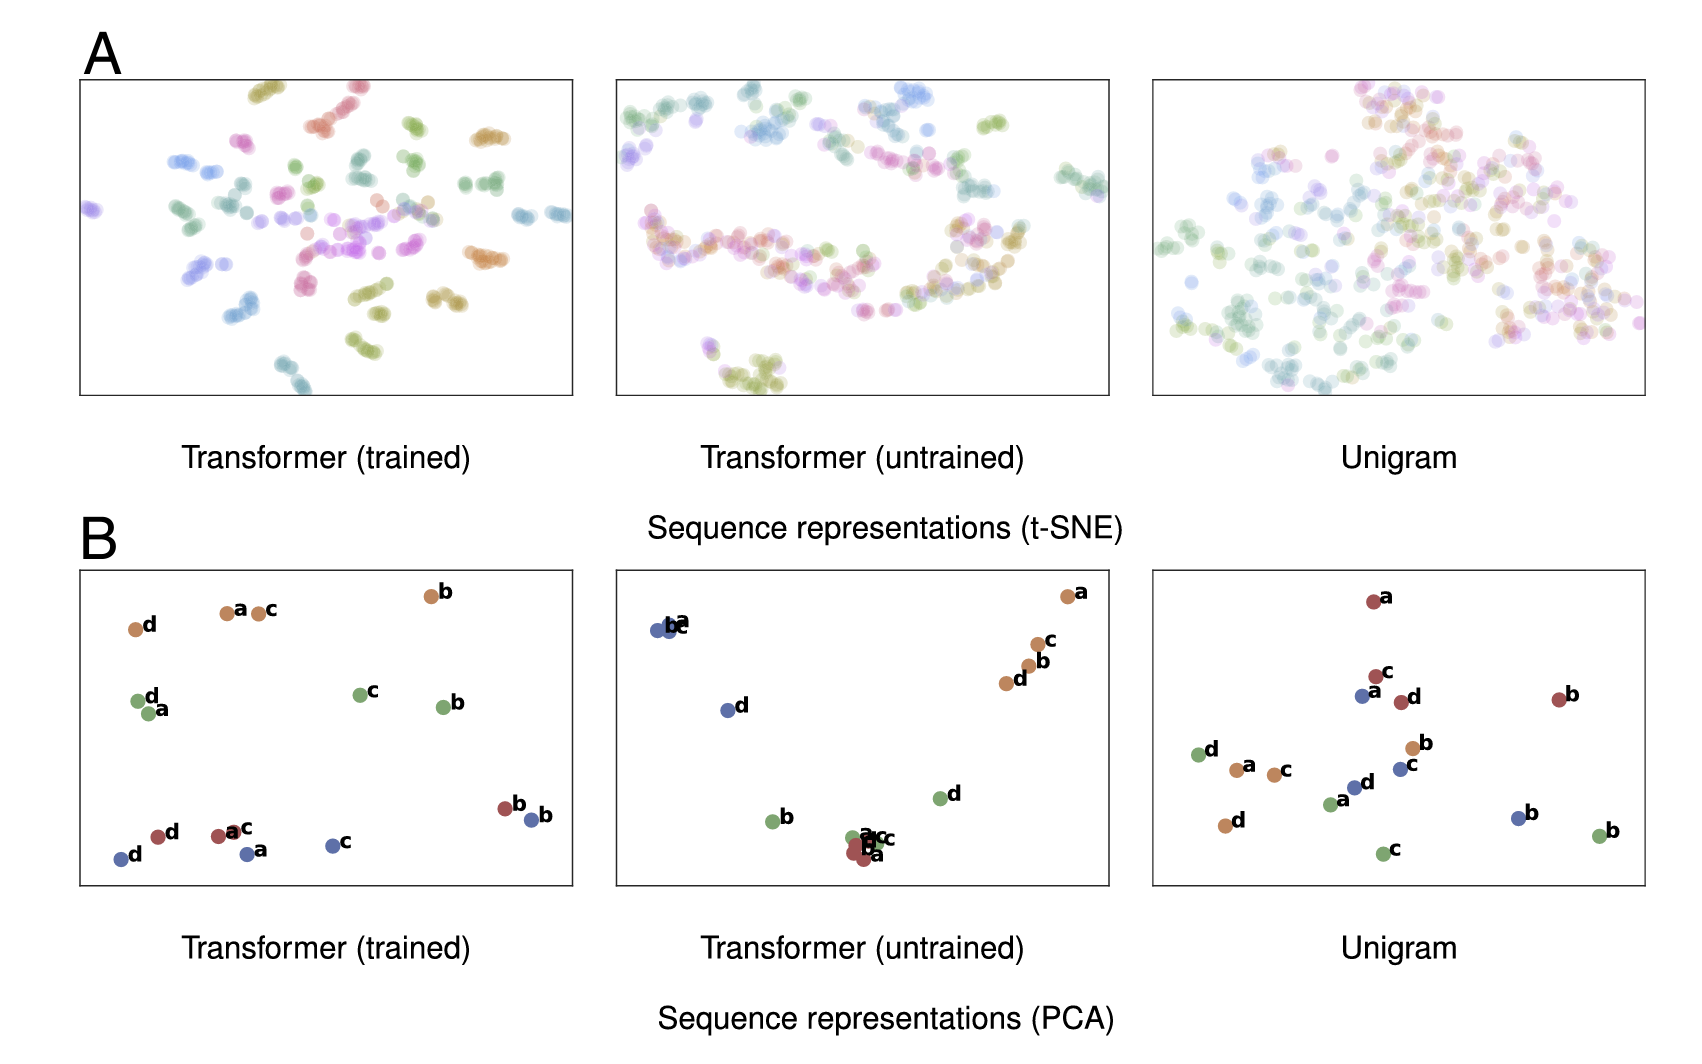
\includegraphics[width=\linewidth]{img/gene-tsne.png}
    \caption{Species and orthology become principal axes of variation, indicating that unsupervised learning captures biological variations.}
    \label{fig:gene-tsne}
\end{figure}
    


\section{Predicting the effects of genetic variants and mutations with Enformer}
The Enformer model by Avšec et al.~\cite{avsec_effective_2021} utilizes transformer modules, known for their effectiveness in natural language processing, to analyze DNA sequences. Its key features include:
\begin{itemize}
    \item Transformer Layers: These enable the model to consider each part of the DNA sequence in relation to the entire sequence, crucial for integrating distant genomic elements.
    \item Extended Receptive Field: Enformer can analyze elements up to \textbf{100 kb} from the transcription start site, much further than previous models, allowing it to capture a broader range of regulatory elements like distant enhancers.
    \item Attention Mechanism: This allows the model to weigh different parts of the sequence differently, depending on their relevance to gene expression.
\end{itemize}
By utilizing existing gene expression data, Enformer can be adapted to Dicty's genome, enabling predictions of gene expression levels based on genomic sequences.

\subsection{Effects of genetic variants}

Enformer is a computational model that can predict the effects of genetic variants on gene expression in a cell-type-specific manner, which is valuable for fine-mapping noncoding associations from genome-wide association studies (GWAS). Figure~\ref{fig:variant} depicts Enformer's predictive analysis of a genetic variant (rs11644125 C/T) showing its impact on NLRC5 gene expression, with model predictions suggesting the T allele reduces expression, possibly through altered SP1 transcription factor binding, as validated by cap analysis gene expression (CAGE) data in peripheral blood mononuclear cells (PBMCs).
\begin{figure}[ht]
\centering
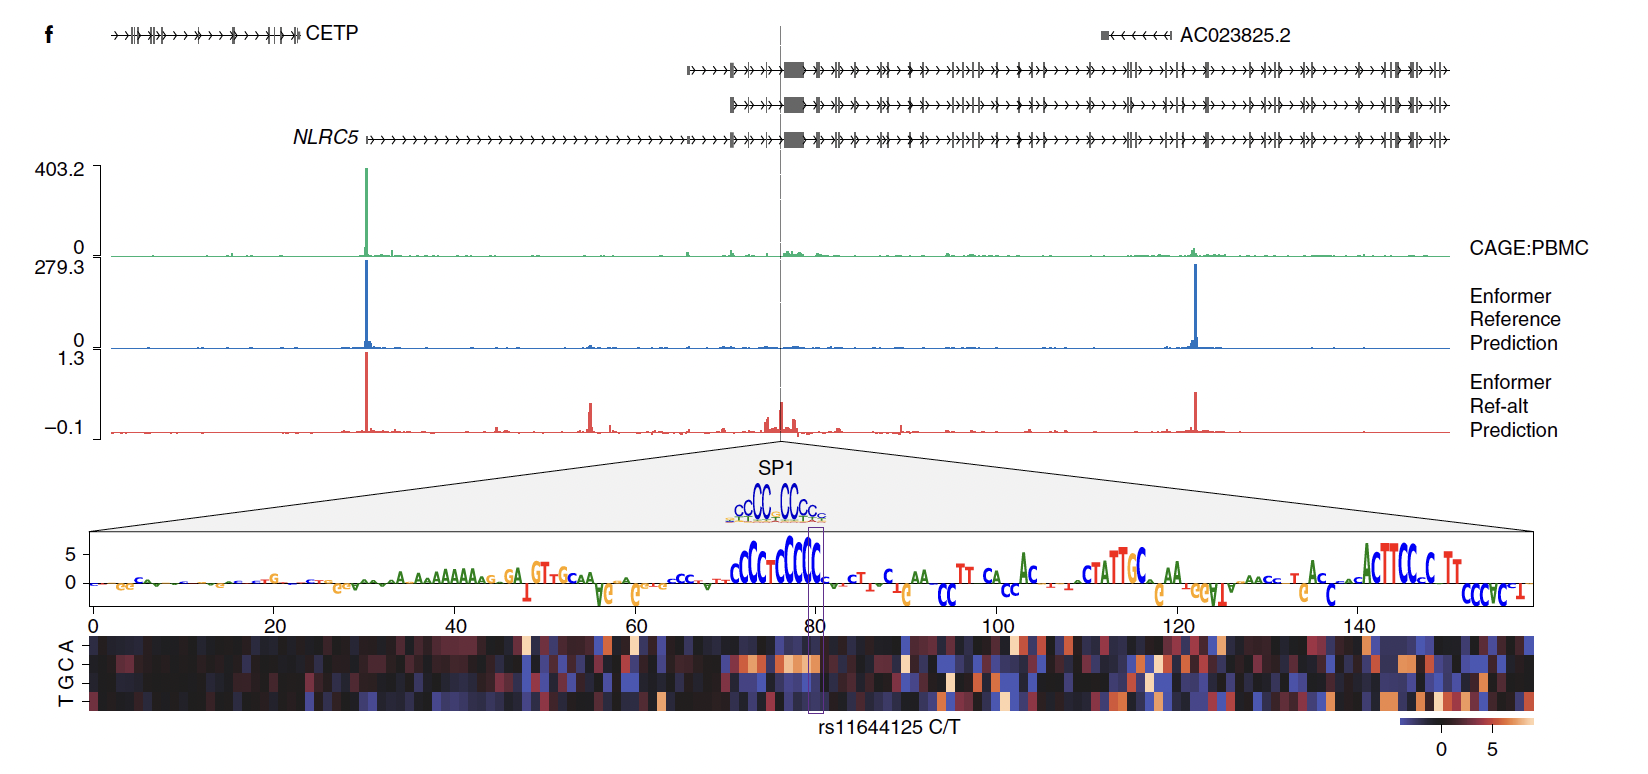
\includegraphics[width=\linewidth]{img/variant.png}
\caption{Enformer predicts that the T allele of variant rs11644125 decreases NLRC5 expression, likely by affecting SP1 binding, corroborated by CAGE data in PBMCs.}\label{fig:variant}
\end{figure}

\subsection{Effects of mutations}
Enformer showcased superior prediction capabilities for the functional effects of genetic variants, outperforming other methods in a massively parallel reporter assay (MPRA) dataset by using a lasso regression model that incorporated Enformer predictions as features. Enformer outperforms other methods in variant effect prediction by showing consistently higher Pearson correlation values across different genetic targets and cell types \ref{fig:mutations}.

\begin{figure}[ht]
    \centering
    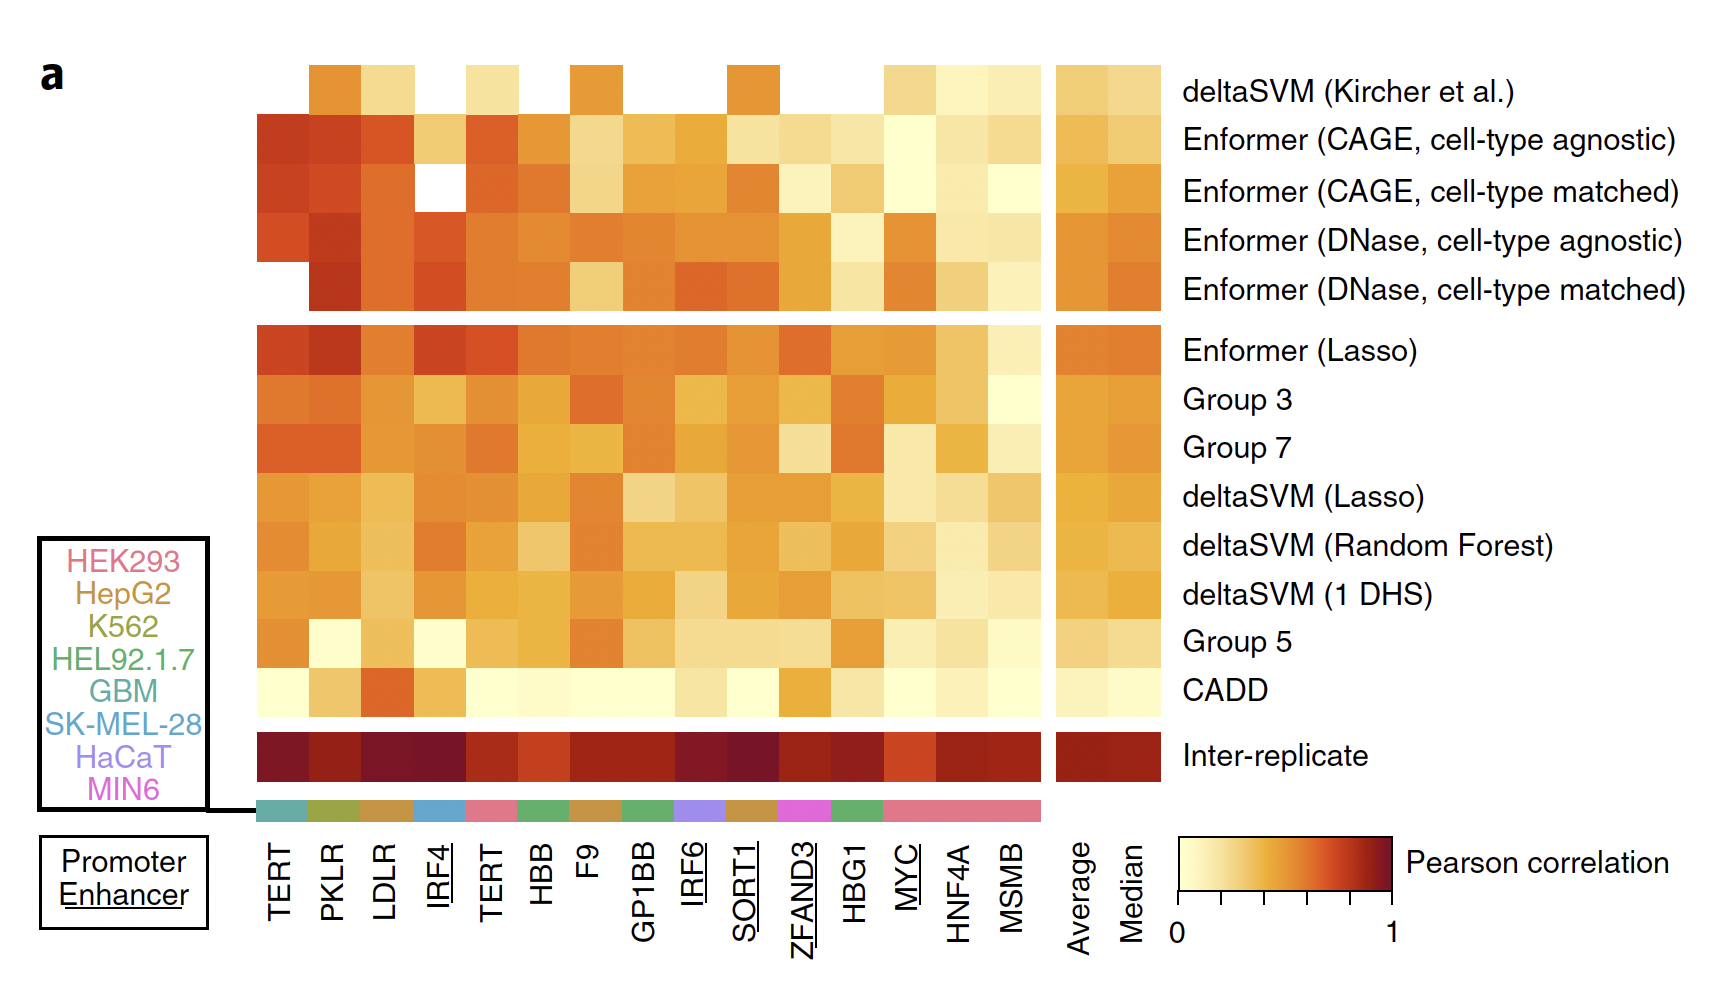
\includegraphics[width=\linewidth]{img/mutations2.png}
    \caption{Enformer demonstrates high Pearson correlation coefficients across multiple cell lines and target loci, indicating superior performance in predicting the functional effects of genetic variants compared to other methods such as deltaSVM.}\label{fig:mutations}
\end{figure}



\bibliographystyle{unsrt} 
\bibliography{sample}
\end{document}

\endinput
%%
%% End of file `elsarticle-template-harv.tex'.
